\chapter{Ergebnisse}
In diesem Kapitel werden zu Beginn
Eigenschaften der Floquet Theorie an dem Modell überprüft.
Weiterhin wird die zeitliche Entwicklung
eines Zustandes durch den
Floquet Formalismus mit der einer numerischen Lösung der
Schrödingergleichung verglichen.
Auf zwei unterschiedliche Weisen wird jeweils ein in der Zeit
gemittelter Strom berechnet und miteinander verglichen.
Anschließend soll das System auf zwei Elektronen erweitert und ein Strom berechnet werden.
In den folgenden Rechnungen wird der Sprungterm $J=1$
gesetzt und  alle Ergebnisse in Einheiten von $J$ angegeben.
Zusätzlich wird in atomaren Einheiten gerechnet, folglich gilt:
\begin{align}
   \symup{e}=\hbar=\text{m}_\symup{e}=1.
\end{align}
\section{Frequenzabbhängigkeit der Quasienergien}
Zunächst werden die Eigenschaften der Floquet Theorie
untersucht. Dafür
werden die Eigenwerte
 $\epsilon_{\alpha n}$ für eine
Matrix $\mathcal{H}_\mathrm{F}$ mit der
Größe $N=1$, konstanter lokaler Energie $a=1$ und E-Feldamplitude $E_0=1$
für Frequenz in einem Bereich von $0-6$  berechnet.
Um die Effekte der Störung $V(t)$ zu verdeutlichen,
werden ebenfalls Eigenwerte $E_{\alpha n}$ für Matrix $\mathcal{H}_F$ mit $E_0=0$, dies besschreibt den
zeitunabhänigen Fall, berechnet, sodass in Abbildung \ref{fig:epsilon_f}
die berechneten Eigenwerte verglichen werden können.

\begin{figure}
   \centering
   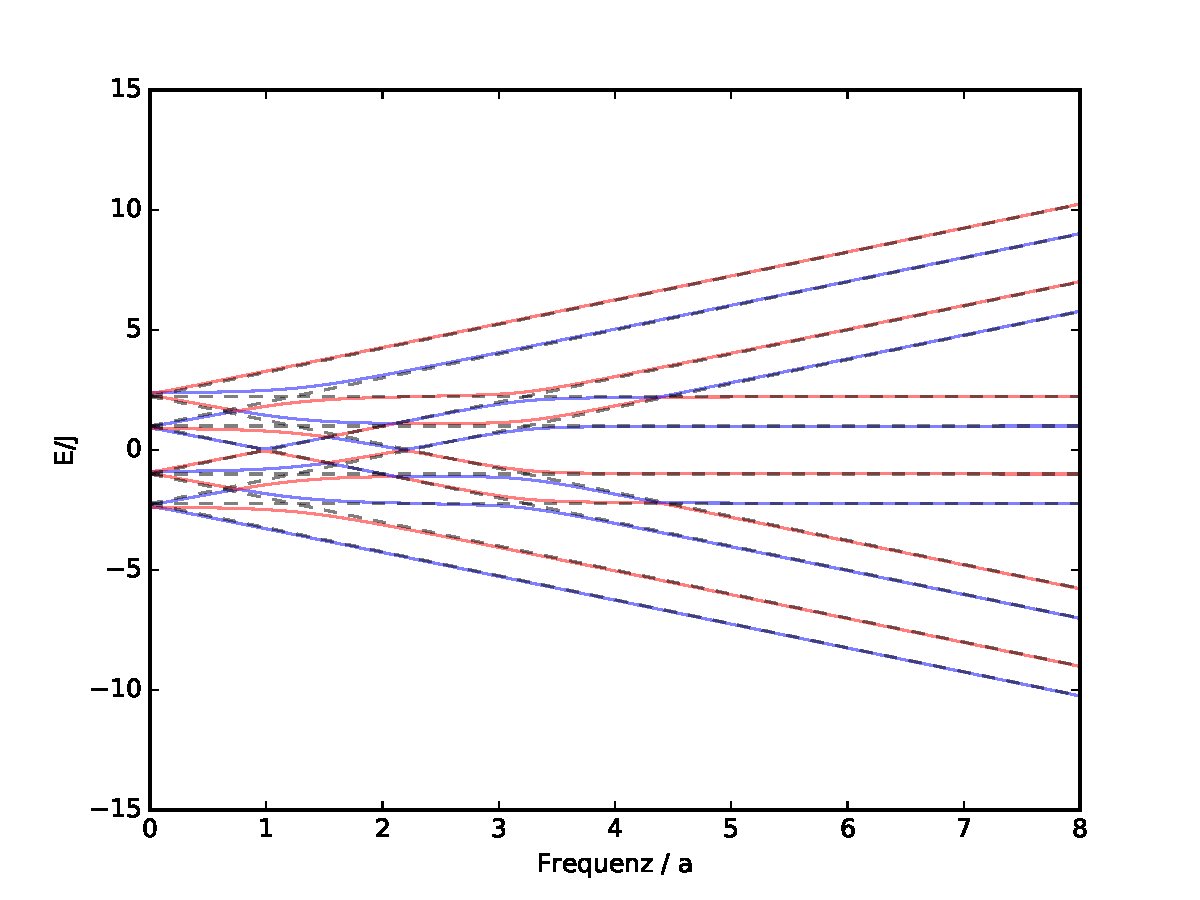
\includegraphics[width=0.7\textwidth]{Programme/Freqenzen_kontinuierlich/Plots/Plot_fur_a=1.0_E=1.0.pdf}
   \caption{Eigenwerte $\epsilon_{\alpha n}$ der Matrix $\mathcal{H}_\mathrm{F}$ für $a=1$ und $E_0=1$ und
   Eigenwerte $E_{\alpha n}$ des zeitunabhängigen System in Abhängigkeit von der Frequnez $\omega$.}
   \label{fig:epsilon_f}
\end{figure}
In der Abbildung \ref{fig:epsilon_f} können, wie in \cite{haenggi} beschrieben, an Stellen der Überschneidung der Eigenwerte  $E_{\alpha n}$
des zeitunabhängigen Systems die Phänomene des sogenannten "avoided crossing" und
"exact crossing" der Quasienergien $\epsilon_{\alpha n}$ beobachtet werden,
die durch das zeitabhängige elektrische Feld hervorgerufen werden.
Dies dient hier nur als Bestätigung der Funktionsweise
des aufgestellten Algorithmus für die Matrix-Methode und wird im Folgendem nicht weiter behandelt.

\section{Brillouin-Zone der Quasienergien}
In dem Abschitt wird versucht, die Quasienergien, wie in
\ref{sec:flotheo} beschrieben, in einer Art
 Brillouin-Zone darzustellen.
Dafür werden Quasienergien bei einer konstanten Frequenz $\omega=1$ und
lokalen Energie $a=1$ in Abhängigkeit der
Amplitude $E_0$, die hier unabhängig
von realistischen Werten zur besseren Veranschaulichung im
Bereich von $0$ bis $6$ liegt, berechnet.
Diese sind in der Abbildung \ref{fig:brillouin} gegen $E_0$ aufgetragen.
Zusätzlich wird die Größe $N$ der Matrix $\mathcal{H}_F$ variiert.

\begin{figure}
  \centering
  \begin{subfigure}{0.48\textwidth}
    \includegraphics[width=1\textwidth]{Programme/Energien_kontinuierlich/Plots/Plot_fur_a=1.0_w=1.0N=1.0.pdf}
    \caption{N=1}
    \label{fig=N_1}
  \end{subfigure}
  \begin{subfigure}{0.48\textwidth}
    \includegraphics[width=1\textwidth]{Programme/Energien_kontinuierlich/Plots/Plot_fur_a=1.0_w=1.0N=3.0.pdf}
    \caption{N=3}
    \label{fig=N_3}
  \end{subfigure}
  \begin{subfigure}{0.48\textwidth}
    \includegraphics[width=1\textwidth]{Programme/Energien_kontinuierlich/Plots/Plot_fur_a=1.0_w=1.0N=6.0.pdf}
    \caption{N=6}
    \label{fig=N_6}
  \end{subfigure}
  \begin{subfigure}{0.48\textwidth}
    \includegraphics[width=1\textwidth]{Programme/Energien_kontinuierlich/Plots/Plot_fur_a=1.0_w=1.0N=10.0.pdf}
    \caption{N=10}
    \label{fig=N_3}
  \end{subfigure}
  \caption{Berechnete $\epsilon_{\alpha n}$ für unterschiedliche Größen der Matrix $\mathcal{H}_F$
  bei einer lokalen Energie $a=1$ und einer Frequenz $\omega=1$ in der 1. und 2. Brillouin Zone}
  \label{fig:brillouin}
\end{figure}

Deutlich wird, dass ein zu kleines $N$ der Bedingung für eine Darstellung in der Brillouin-Zone nicht genügen.
Jedoch können für ein ausreichend große $N$ die Quasienergien $\epsilon_\alpha$ in die erste Brillouin-Zone
mit $-\frac{\omega}{2}<\epsilon_\alpha<\frac{\omega}{2}$ dargestellt und
alle anderen Quasienergien $\epsilon_{\alpha n}$ durch die Periodizitätsbedingung \eqref{eqn:epsilon_n} berechnet werden.
In der ersten Brillouin-Zone der Abbildung \ref{fig:brillouin} existieren genau vier Quasienergien, folglich besitzt das System
ebenfalls vier Quasienergien und vier Quasizustände.
%Aus der  Abbildung \ref{fig:brillouin} kann entnommen werden, System vier Quasienergien besitzt
Es kann jedoch selbst bei größerem $N$ beobachtet werden, dass bei höheren Brillouin-Zonen?? die Periodizität nicht mehr gegeben ist.

\section{Orthogonalität der Quasizustände}
Im Folgenden soll die Orthogonalität zwischen den Quasizuständen $\ket{\Phi_\alpha}$ aus der Gleichung \eqref{eqn:ortho} für
unterschiedliche Größen der Matrix $\mathcal{H}_F$ überprüft werden.?? Die Quasizustände $\ket{\Phi_\alpha}$ berechnen sich jeweils aus
den zu $\epsilon_\alpha$ zugehörigen Eigenvektoren. Indem die Komponenten der Eigenvektoren als $c_{\alpha,k}^{n}$ verwendet werden,
ergeben sich aus Gleichung \eqref{eqn:PHI} die Quasizustände des Systems.??
In der Abbildung \ref{fig:ortho} ist das Skalarprodukt zwischen den Quasizuständen in Abhängigkeit von der Größe $N$ der Matrix
$\mathcal{H}_F$ dargestellt.
Dies soll für die später verwendete Größen $a=0,5$ , $E_0=0,1$  und $\omega=1$ überprüft werden.
.

\begin{figure}
    \centering     % vielleicht mit 2x2 subfigure
    \includegraphics[width=0.7\textwidth]{Programme/Orthogonalitat_der_quasizustande/Plots/Potential=0.5/Energie=0.1/Frequenz=1.0/Plot_fur_phi1_phi_i}
    \caption{Das Skalarprodukt $\braket{\Phi_1|\Phi_i}$ folgt auch für die anderen Zustände}
     \label{fig:ortho}
\end{figure}

Aus der Abbildung \ref{fig:ortho} kann entnommen werden, dass bei zu geringem $N$ die Orthogonalität der Quasizustände
nicht gegeben ist.
In diesem Fall erweist sich eine Größe von $N=5$ als ausreichend zur Gewährleistung der Orthogonalität.
Es kann ebenfalls eine (ein Anitproportionle )Abhängigkeit von lokaler Energie $a$ und Frequenz $\omega$ beobachtet werden.
Für Kleinerwerden der jeweiligen Größe wird ein größeres $N$ benötigt.
Antiproportional????
Somit ist es notwendig,
bei den folgenden Berechnungen die
Orthogonalität der Quasizustände für
Werte von $\omega$ und $a$ kleiner als die in Abbildung
\ref{fig:ortho} gewählten Größen stehts zu überprüfen.
Andernfalls reicht eine Matrixgröße von $N=5$ zum Erfüllen der Bedingung aus.



% -über formel .. kann quasizustand berechnet werden
% -die Orthogonalitäts bedingung formel .. sollte erfüllt sein

\section{Zeitentwicklung eines Zustandes durch den Floquet Formalismus}
In diesem Abschnitt wird eine Zeitentwicklung des Ein-Elektron-Systems mit oszillierendem E-Feld durch den Floquet Formalismus durchgeführt.
Als Startzustand $\ket{\Psi_0}$ wird der Grundzustand $\ket{\phi_1}$ des zeitunabhänigen Systems verwendet, da davon
ausgegangen werden kann, dass das System zu Beginn im energieärmsten Zustand verweilt.
Es sollen zunächst nur Frequenzen $\omega$ des E-Feldes
betrachtet werden, die nicht einer Resonanzfrequenz entsprechen.
In der Abbildung \ref{fig:Resonanz} sind
 die Resonanzfrequenzen \eqref{eqn:Resonanz} in Abhängigkeit
von den lokalen Energien aufgetragen.

\begin{figure}
  \centering
  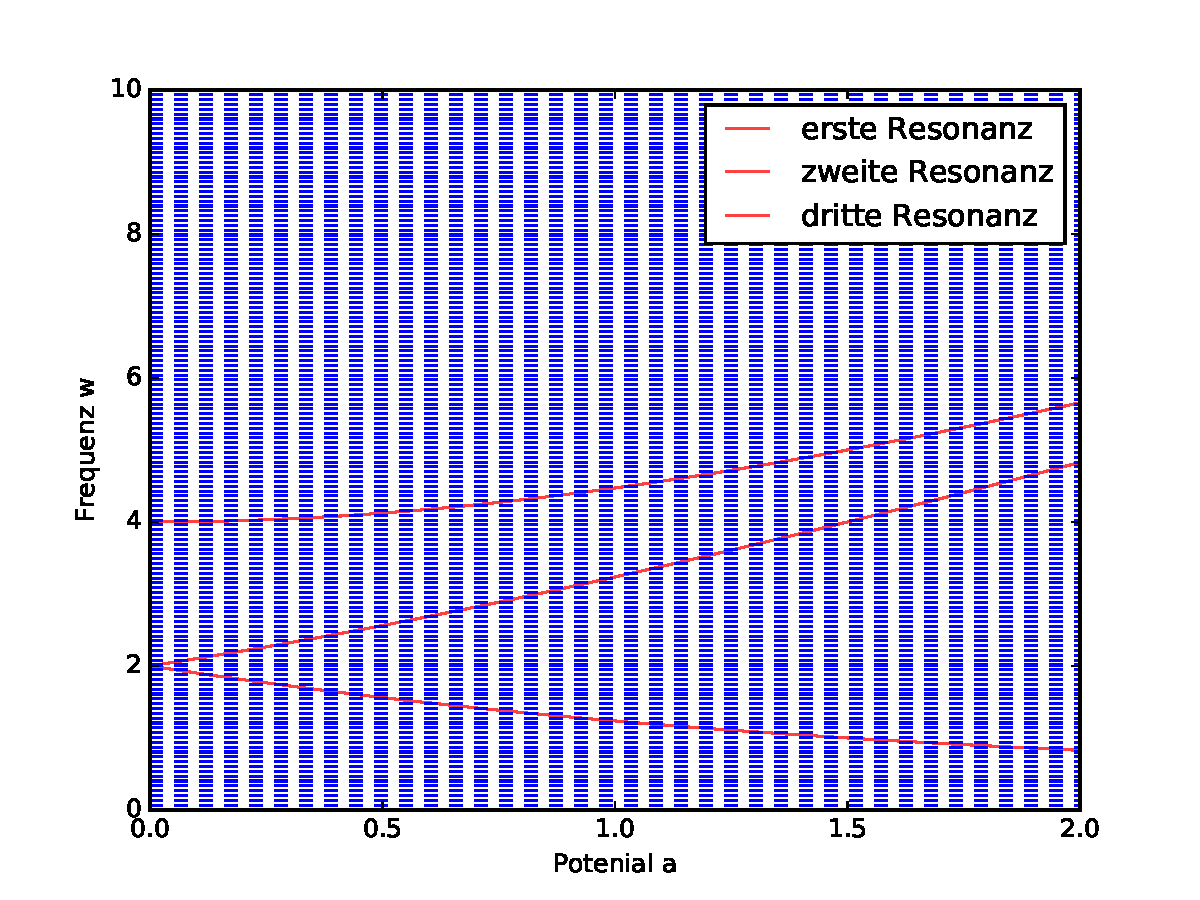
\includegraphics[width=0.7\textwidth]{Programme/Eigenzustande/Plots/Resonanzen.pdf}
  \caption{Resonanzfrequenzen in Abhängigkeit von der lokalen Energie $a$}
  \label{fig:Resonanz}
\end{figure}


Unter dem Ausschluss der Resonanzfrequenzen aus der
 Abbildung \ref{fig:Resonanz}, wird bei einer lokalen Energie
$a=0,5$ und einer Amplitude $E_0=0,1$ die Frequenz $\omega=1$ gewählt.
Um die Zeitentwicklung nach Floquet durchführen zu können, muss
zunächst, wie in Gleichung \eqref{eqn:superposition} beschrieben, der Grundzustand
als Superposition der Quasizustände ausgedrückt werden.
Durch Anwenden des Zeitpropagators \eqref{eqn:Propagator} auf den Grundzustand,
 ist es somit möglich den zeitentwickelten Grundzustand
$\ket{\Psi(t)}$ zu berechnen.

In der Abbildung \ref{fig:zeitentwicklung} ist
die Aufenthaltswahrscheinlichkeit
$\lvert\braket{e_i|\Psi(t)}\rvert^2$ für
die vier unterschiedlichen Gitterplätze in Abhängigkeit von der Zeit dargestellt.
Dabei wird ebenfalls eine numerische Lösung
der Schrödingergleichung für den Grundzustand durch den
adaptiven Algorithmus $\textit{lsode}$,
der durch das Programm Octave \cite{octave}bereitgestellt wird, aufgetragen.

\begin{figure}
  \centering
  \includegraphics[width=0.7\textwidth]{Programme/Eigenzustande/Plots/Potential=0.5/Energie=0.1/Besetzungen(t)_mit_Floquet_N=5w=1.0.pdf}
  \caption{Zeitenwicklung des Grundzustandes}
  \label{fig:zeitentwicklung}
\end{figure}

Es zeigt sich, dass die verschiedenen Lösungen übereinstimmen. Somit kann die Lösung der Floquet Theorie bestätigt werden.
Auffällig ist, dass die Gitterplätze $1$ und $3$
bevorzugt sind, dies kann durch die Struktur des Bandisolators begründet werden, da
die beiden Position eine geringere lokale Energie $a$ besitzen.
%
% -wenn Zustände orthogonal zeitentwicklung möglich
% -vergleich mit lsode
% -stimmt überein eignet sich folglich für zeitentwicklung

\section{Strom im System}
In dem vorigen Abschnitt konnte die Zeitentwicklung der Floquet Theorie betätigt werden.
Diese wird hier genutzt zur Berechnung des Stromes in dem System.
Durch
\begin{align}
\braket{\mathcal{J}}(t)=\braket{\psi(t)|  \mathcal{J}|\psi(t)}
\intertext{mit dem Strom(dichte)operator\cite{schwabl}}
\mathcal{J}= -\frac{\text{i}\symup{e}}{4} C \sum_i^4 c_{i+1}^\dag c_{i}^{\phantom{\dag}}  -c_{i}^\dag c_{i+1}^{\phantom{\dag}}
\end{align}
ergibt sich der Stromfluss des Systems.
Wird $\ket{e_i}$ wieder als Basis gewählt, ergibt sich
die Matrixdarstellung des Strom(dichte)operators
\begin{align}
\mathcal{J}=\frac{\symup{i}\symup{e}}{4}\begin{pmatrix}
  \phantom{-}0&           -C &\phantom{-}0 & \phantom{-}C \\
          C   & \phantom{-}0 &         -C  & \phantom{-}0\\
  \phantom{-}0& \phantom{-}C &\phantom{-}0 &           -C \\
            -C& \phantom{-}0 &\phantom{-}C & \phantom{-}0
\end{pmatrix}.
\end{align}
Die Konstante $C$ wird ebenfalls auf $1$ gesetzt und
die Ergebnisse in Einheiten von $C$ angegeben.
Die Abbildung \ref{fig:strom_t} enthält den Stromfluss des Systems in Abhängigkeit von der Zeit.

\begin{figure}
  \centering
  \includegraphics[width=0.7\textwidth]{Programme/Strom/Plots/Potential=0.5/Energie=0.1/Stromerwartungswert(t)_N=5w=1.0.pdf}
  \caption{Strom im System in Abhängigkeit der Zeit}
 \label{fig:strom_t}
\end{figure}



Die Messung  des Stromes $\braket{\mathcal{J}}(t)$ auf so kleinen Zeitskalen ist jedoch nicht möglich, daher
misst der Beobachter nur einen in der Zeit gemittelten Strom
\begin{align}
  \bar{\braket{\mathcal{J}}}= \frac{1}{T}\int_0^T \braket{\Psi(t)|\mathcal{J}|\Psi(t)}.
\end{align}
Mit Hilfe des Zeitpropagators \eqref{eqn:prop} ist es in dem Floquet Formalismus problemlos möglich, zeitlich
gemittelte Erwartungswerte von
Operatoren zu berechnen.
Das zeitliche Mittel über eine große Zeitspanne??? eine Periode $T$ ist gegeben durch
\begin{align}
  \bar{\braket{O}}= \frac{1}{T}\int_0^T \braket{\Psi(t)|O|\Psi(t)}.
\intertext{Durch Einsetzen von \eqref{eqn:psi_t} und \eqref{eqn:fourier}
 ergibt sich}
 \bar{\braket{O}}&= \sum_\alpha \lvert c_\alpha \rvert^2  \sum_{-\infty}^{\infty} \braket{c_\alpha^n\lvert O \rvert c_\alpha^n}  \label{eqn:mittel} \text{\cite{gespräch}}
 \intertext{mit}
  c_\alpha&=\braket{\Psi_0\vert\Phi_\alpha}
\end{align}
nach Ausführung der Integration.
??In dem Floquet Formalismus ist es somit nicht notwendig die Erwartungswerte
 zu berechnen und diese über eine
Zeitspanne zu mitteln. Durch die Formel \eqref{eqn:mittel} kann
der gemittelte Erwartungswert unkompliziert berechnet werden.??
Zur Überprüfung der Gleichung \eqref{eqn:mittel} wird
der gemittelte Stromerwartungswert $\bar{\braket{\mathcal{J}}}$
für unterschiedliche Frequenzen $\omega$
in Abhängigkeit von der Amplitude des elektrischen Feldes $E_0$
zum einen durch die Gleichung \ref{eqn:mittel}
und zum anderen über die Mittelung über eine
lange Zeitspanne, hier
T=??,  ??mehrere Perioden?? des berechneten
Erwartungswert des Stromes $\braket{\mathcal{J}}(t)$ bestimmt.
Die Abbildung \ref{fig:E_Strom} enthält jeweils die aus
den zwei verschiedenen Methoden für $a=0,5$
berechneten gemittelten Ströme $\bar{\braket{\mathcal{J}}}$.


\begin{figure}
  \centering
  \includegraphics[width=0.7\textwidth]{Programme/Strom_mittelwerte/Plots_mittelwerte/Potential=0.5Stromerwartungswert(t)_N=5.pdf}
  \caption{mittelwert des Stromerwartungswert für die zweite Methode wurde über eine Zeit Spanne von ?? gemittelt }
  \label{fig:E_Strom}
\end{figure}


Aus der Abbildung \ref{fig:E_strom} kann entnommen werden,
dass die Gleichung \ref{eqn:mittel} identische
Ergebnisse wie die zweite Methode liefert.
Somit ist bestätigt, dass der zeitlichgeittel
Stromerwartungswert $\bar{\braket{\mathcal{J}}}$
über die Gleichung \ref{eqn:mittel}
berechnet werden kann.
Im Folgenden wird ??(nur) die Methode,
die die Floquet Theorie bereitstellt,
um zeitlich gemittelte Stromerwartungswerte zu berechnen,
verwendet.

\section{Strom Abhängigkeiten}
Wie in dem Kapitel \ref{sec:inverfaraday} beschrieben,
soll der Strom bei dem IFE??(Inverser Faraday Effekt)
in einem Isolator quadratisch
mit der Amplitude des elektrischen Feldes $E_0$
sowie linear mit der Frequenz $\omega$ des elektrischen
Feldes steigen. Diese Abhängikeiten sollen nun für den
 Ein-Elektronen-Fall überprüft werden.
Für die quadratische Abhängigkeit wird in der Abbildung
\ref{fig:E_abb} der zeitliche Strommittelwert $\bar{\braket{\mathcal{J}}}$
 gegen $E_0$ aufgetragen.
Genutzt werden
vier Frequenzen, die jeweils zwischen den Resonanzen liegen, um Resonanzeffekte zu vermeiden.
Es wird eine lokale Energie von $a=0,5$ und Frequenzen von $\omega=1,2,3,5$,
die jeweils die Bedingung erfüllen, verwendet.
An die berechneten Werte wird versucht eine quadratische Funktion $f(x)=ax^2$
anzulegen\footnote{Mit Hilfe von python \textit{curvefit} }, ebenfalls zu sehen
in Abbildung \ref{fig:E_abb}.

\begin{figure}
  \centering
  \includegraphics[width=0.7\textwidth]{Programme/Strom_fit_e/Plots_mittelwerte/Potential=0.5Stromerwartungswert(t)_N=5.pdf}
  \caption{Überprüfung der $E_0$ abhängigkeiten.}
  \label{fig:E_abb}
\end{figure}

Es ist möglich, eine quadratische Funktion anzulegen,
folglich kann die quadratische Abbhängigkeit
bestätigt werden.

Abschließend gilt es, die Linearität des Strommittelwertes
 zu der Frequenz zu untersuchen.
Hierfür wird der Strommittelwert $\bar{\braket{\mathcal{J}}}$
in Abhängigkeit von der Frequenz $\omega$ in einem
Bereich von $0$ bis $8$ für
zwei verschiedene elektrische Amplituden $E_0=??,??$
untersucht, siehe Abbildung \ref{fig:I_freq}.
Erneut wird eine lokale Energie von $a=0,5$???? variieren ???? verwendet.

\begin{figure}
   \centering
   \includegraphics[width=0.7\textwidth]{Programme/Strom_frequenzabb/Plots_mittelwerte/Potential=0.5Stromerwartungswert(t)_N=5.pdf}
   \caption{Strom in Abhängigkeit von der Frequenz}
   \label{fig:w_abb}
\end{figure}


In der Abbildung können Resonanzeffekte
bei den zuvor berechneten Resonanzfrequenzen
beobachtet werden. Auf Grund der
dominierenden Resonanzeffekte in Abbildung \ref{fig:w_abb}
lässt sich die Linearität nicht eindeutig bestätigen.
Um die Resonanzeffekte zu ??vernächlässigen??, soll ein kleinerer Frequenzbereich, hier von
$0-0,8$, untersucht werden.
Jedoch fällt der Strom in diesem Bereich ??'unnormal'??
ab. Als Ursache hierfür kann eine in diesem
Frequenzbereich nicht mehr gewährleistete Orthogonalität der
Quasizustände sein, da zuvor nur eine minimale Frequenz
von $\omega=1$ auf Orthogonalität überprüft wurde.
Um dies zu untersuchen, wird das Skalarprodukt der Quasizustände gegen
die Frequenz \omega in der Abbildung \ref{fig:N_5} für $N=5$ aufgetragen.
%Dies geschieht ebenfalls für  $N=10$, $N=20$ und $N=50$

\begin{figure}
   \centering
   \begin{subfigure}{0.48\textwidth}
       \includegraphics[width=1\textwidth]{Programme/Orthogonalitat_der_quasizustande_frequenz/Plots/Potential=0.5/Energie=0.1/Anzahl=5/Plot_fur_phi1_phi_i.pdf}
       \caption{N=5}
       \label{fig:N_5}
     \end{subfigure}
     \begin{subfigure}{0.48\textwidth}
       \includegraphics[width=1\textwidth]{Programme/Orthogonalitat_der_quasizustande_frequenz/Plots/Potential=0.5/Energie=0.1/Anzahl=10/Plot_fur_phi1_phi_i.pdf}
       \caption{N=50}
       \label{fig:N_10}
     \end{subfigure}
     \begin{subfigure}{0.48\textwidth}
       \includegraphics[width=1\textwidth]{Programme/Orthogonalitat_der_quasizustande_frequenz/Plots/Potential=0.5/Energie=0.1/Anzahl=20/Plot_fur_phi1_phi_i.pdf}
       \caption{N=50}
       \label{fig:N_20}
     \end{subfigure}
     \begin{subfigure}{0.48\textwidth}
       \includegraphics[width=1\textwidth]{Programme/Orthogonalitat_der_quasizustande_frequenz/Plots/Potential=0.5/Energie=0.1/Anzahl=50/Plot_fur_phi1_phi_i.pdf}
       \caption{N=50}
       \label{fig:N_50}
     \end{subfigure}
        \caption{Das Skalarprodukt }
    \label{fig:N_gross}
\end{figure}


Die Abbildung \ref{fig:N_5} bestätigt
die Vermutung der fehlenden Orthogonalität.
Folglich muss die Größe $N$ der Matrix
$\mathcal{H}_F$ erhöht werden.
Die Abbildung \ref{fig:N_gross} enthält ebenfalls
den gleichen Zusammenhang
aus \ref{fig:N_5} jedoch für
größere $N$.
Es zeigt sich, dass für höhere $N$ geringere Frequenz
erreicht werden können, welche die orthogonalität Bedingung
erfüllen. Allerdings
ist der Zusammenhang ?'noch nicht klar'?(Antiproportional).
Als Konsequenz folgt, dass für geringere
Frequenzen die Matrix zu groß wird und nicht
mehr unkompliziert diagonalisierbar ist.
Demzufolge ist es notwendig, bei Untersuchung des linearen Bereiches eine
größere Matrix $\mathcal{H}_F$ aufzustellen. Hier soll $N=50$ genügen,
folglich dürfen Frequenzen kleiner als $0,1??$ bei der Überprüfung der Linearität nicht
berücksichtigt werden.
Der Strommittelwert $\bar{\braket{\mathcal{J}}}$
 wird im zuvor geforderten Frequenzbereich $0-0,8$
gegen $\omega$ aufgetragen, siehe Abbildung \ref{fig:geraden_fit}.
Bei Frequenzen um $0,7??$
machen sich bereits Resonanzeffekte bemerkbar,
deshalb wird versucht eine Gerade im Frequenzbereich $0,1??$-$0,5??$
an die berechneten Werte anzupassen. ??Fitten??.

\begin{figure}
    \centering
    \includegraphics[width=0.7\textwidth]{Programme/Strom_geraden_fit/Plots_mittelwerte/Potential=0.5Stromerwartungswert(t)_N=50.pdf}
    \caption{Geraden fit}
    \label{fig:geraden_fit}
\end{figure}

Die berechneten Werte und die Gerade liegen übereinander.
Aufgrund dessen kann der lineare Zusammenhang in diesem Frequenzbereich bestätigt werden.

% -berechung des Stromes
% -überprüfung der quadratischen Ahängigkeit der Stromes
% -frequenz abhängigkeit überprüfen (gerade)
% -für kleine frequenz problem mit orthogonalität

\section{Zwei-Elektronen-System}
Das Modell kann unkompliert auf ein
Zwei-Elektronen-System, indem
das Pauliverbot gilt, erweitert werden.
Die Eigenwerte setzen sich dabei aus
linear Kombination der Eigenwerte
des Ein-Elektron-Systems
zusammen zu
\begin{align}
E_{1/6}=\mp\sqrt{a^2+4J^2}\mp a
E_{2/5}=\mp\sqrt{a^2+4J^2}\mp a
E_{3/4}=0
\end{align}.
Um einen Strommittelwert $\bar{\braket{\symup{J}}}$
in dem Zwei-Elektronen-System,
welches sich im Grunzustand befindet, zu berechnen,
wird der Strommittelwert $\bar{\braket{\symup{J}}}$
für ein Ein-Elektronen-System
sowohl im Grundzustand als
auch im ersten Angeregeten Zustand
berechnet. Aus Addition der beiden
Ein-Elektron-Ströme ergibt sich der Strom
des Zwei-Elektronen-System.
Die Abbildung \ref{fig:2e} enthält
den Strommittelwert des Zwei-Elektronen-Systems
in Abhänigkeit der Amplitude
des Elektrischen Feldes $E_0$.
Wieder wird das System
unterschiedliche Frequenz $\omega=??$
beobachtet.

% \begin{figure}
%     \centering
%     \includegraphics[width=0.7\textwidth]{Programme/Strom_geraden_fit/Plots_mittelwerte/Potential=0.5Stromerwartungswert(t)_N=50.pdf}
%     \caption{Zwei-Elektronen-System}
%     \label{fig:2e}
% \end{figure}
